\chapter{Bibliographie}
\label{cp:bibliographie}

\section{Inertial Measurement Unit}

\paragraph{Un IMU est un dispositif électronique qui mesure et rapporte les données d'accélération linéaire, de vitesse angulaire et d'orientation d'un objet. Les IMU sont largement utilisés dans les applications de navigation inertielle, de robotique et de réalité virtuelle.}

\paragraph{Les IMU sont généralement composés de trois capteurs principaux : un accéléromètre, un gyroscope et un magnétomètre. L'accéléromètre mesure l'accélération linéaire de l'objet, le gyroscope mesure la vitesse angulaire de l'objet et le magnétomètre mesure le champ magnétique terrestre pour déterminer l'orientation de l'objet.}

\paragraph{Les IMU sont souvent utilisés en combinaison avec d'autres capteurs, tels que les GPS et les caméras, pour fournir des données de localisation et d'orientation plus précises. Les IMU sont également utilisés dans les applications de réalité virtuelle pour suivre les mouvements de la tête de l'utilisateur et fournir une expérience immersive.}

\begin{figure}[!htpb]
    \centering
    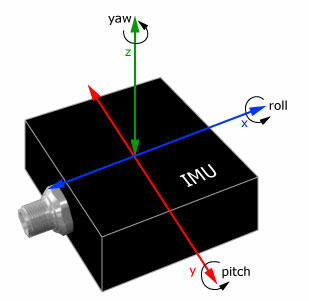
\includegraphics[width=0.5\linewidth]{Figures/imu.jpg}
    \caption[Schéma d'un IMU]{Schéma d'un IMU.}
    \label{fig:imu}
\end{figure}

\subsection{MPU6050}

\paragraph{Le MPU6050 est un IMU à 6 axes qui combine un accéléromètre et un gyroscope dans un seul boîtier. Le MPU6050 est largement utilisé dans les applications de robotique et de contrôle de mouvement en raison de sa petite taille, de sa faible consommation d'énergie et de sa précision élevée. Le MPU6050 est capable de mesurer l'accélération linéaire dans les trois axes et la vitesse angulaire dans les trois axes. Il put communiquer avec un microcontrôleur en utilisant le protocole \gls{i2c} ou \gls{spi}.}

\paragraph*{}
\begin{figure}[!htpb]
    \centering
    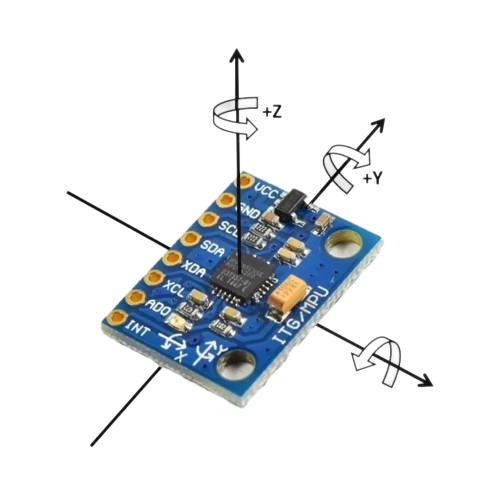
\includegraphics[width=0.8\linewidth]{Figures/mpu6050.png}
    \caption[Module MPU6050]{Module MPU6050.}
    \label{fig:mpu-6050}
\end{figure}


\subsection{I2C}

\paragraph{L'\gls{i2c} est un bus de communication série d'architecture Maitre-esclaves qui permet à plusieurs périphériques de communiquer entre eux à l'aide d'un seul bus de données. L'I2C est largement utilisé dans les applications de capteurs et de contrôleurs pour connecter plusieurs périphériques à un microcontrôleur.}

\paragraph{L'I2C utilise deux fils pour la communication : un fil de données (\acrshort{sda}) et un fil d'horloge (\acrshort{scl}). Chaque périphérique connecté au bus I2C possède une adresse unique qui lui permet de communiquer avec les autres périphériques sur le bus. L'I2C prend en charge plusieurs vitesses de communication, allant de 100 kHz à 3,4 MHz.}

\paragraph*{}
\begin{figure}[!htpb]
	\centering
	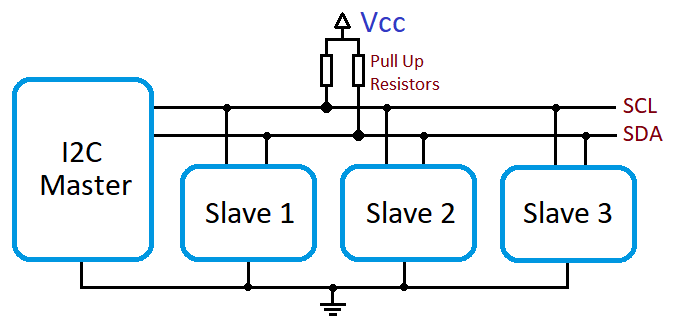
\includegraphics[width=\linewidth]{Figures/i2c.png}
	\caption[Schéma d'un bus I2C]{Schéma d'un bus I2C.}
	\label{fig:i2c}
\end{figure}

\subsection{Paquet I2C}

\paragraph{Un paquet I2C est composé de :}

\begin{enumerate}
	\item \textbf{Condition de demarage :} Un signal de valeur haute sur \acrshort{sda} et \acrshort{scl} indique le début de la communication.
	\item \textbf{Adresse client :} L'adresse du périphérique esclave auquel le maître souhaite communiquer.
	\item \textbf{Ecriture/Lecture :} Un bit de lecture/écriture indique si le maître souhaite lire ou écrire des données. (R = 1, W = 0)
	\item \textbf{Acknowledge :} Un bit de valeur basse sur \acrshort{sda} indique que le périphérique esclave a reçu les données avec succès.
	\item \textbf{Données :} Les données à écrire ou lire.
	\item \textbf{Acknowledge :} Un bit de valeur basse sur \acrshort{sda} indique que le périphérique esclave a reçu les données avec succès.
	\item \textbf{Condition d'arrêt :} Un signal de valeur basse sur \acrshort{sda} et haute sur \acrshort{scl} indique la fin de la communication.
\end{enumerate}

\paragraph*{\textbf{Adresse client} est composé de 7 bits d'adresse et d'un bit de lecture/écriture. Alors que \textbf{les paquets de données} peuvent etre sequentiels composés de 8 bits de données et un bit d'acknowledge entre eux.}

\begin{figure}[!htpb]
	\centering
	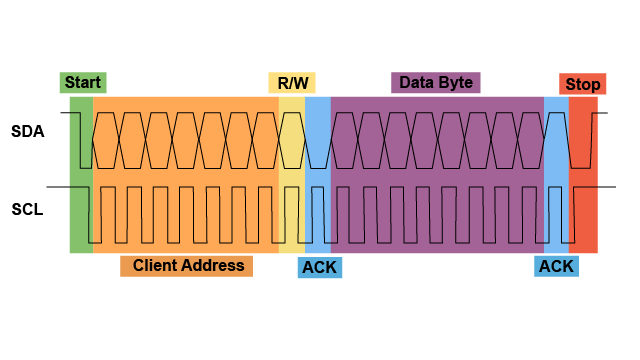
\includegraphics[width=\linewidth]{Figures/i2c-packet.png}
	\caption[Paquet I2C]{Paquet I2C.}
	\label{fig:i2c-packet}
\end{figure}

\section{Electronic Speed Controller}

\paragraph{Un ESC (Electronic Speed Controller) est un dispositif électronique qui convertie DC/AC (DAC) et contrôle la vitesse d'un moteur électrique en ajustant la tension et le courant fournis au moteur. Les ESC sont largement utilisés dans les applications de robotique, de drones et de modélisme pour contrôler la vitesse des moteurs électriques.}

\paragraph{On peut controler la vitesse d'un moteur électrique en ajustant la tension et le courant fournis au moteur. pour varier cette derniere on utilise un signal \acrshort{pwm} (Pulse Width Modulation) qui permet de controler la vitesse du moteur en ajustant la largeur des impulsions du signal.}

\begin{figure}[!htpb]
	\centering
	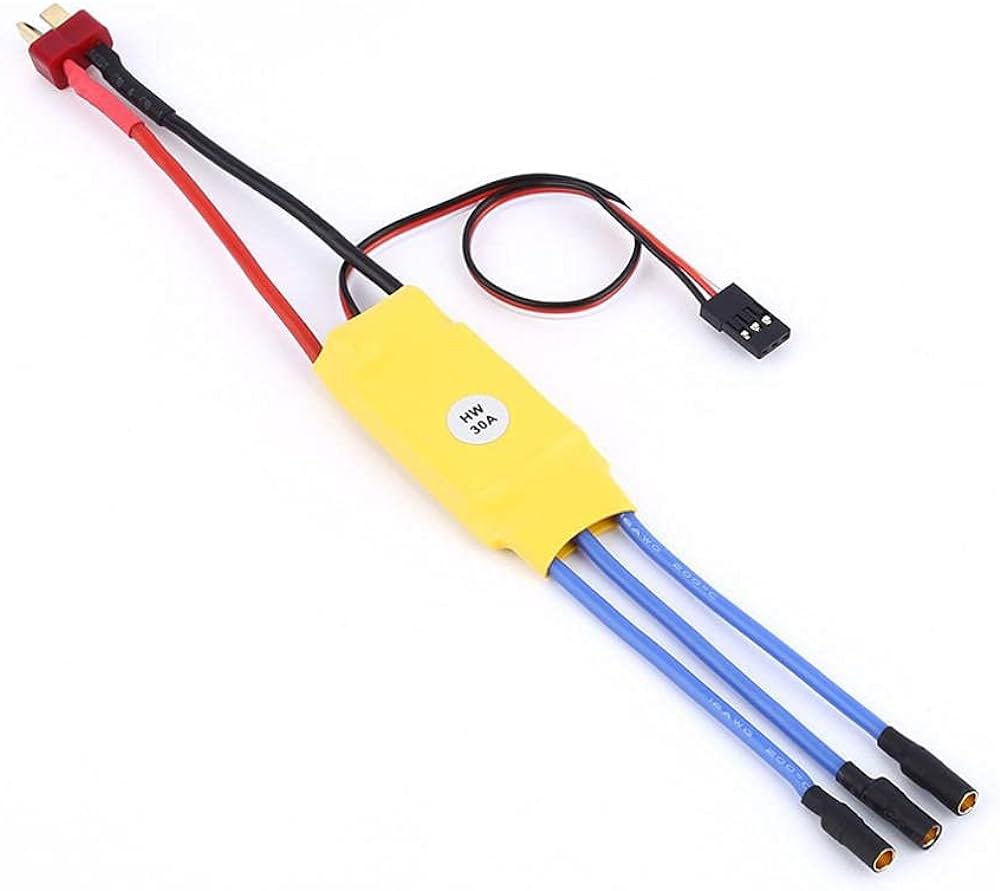
\includegraphics[width=0.7\linewidth]{Figures/esc.jpg}
	\caption[ESC]{ESC.}
\end{figure}

\paragraph{
	On alimente l'ESC avec une tension continue de 5V à 12V, et on controle la vitesse du moteur en ajustant la largeur des impulsions du signal PWM. La largeur de l'impulsion determine la vitesse du moteur, plus l'impulsion est longue, plus la vitesse du moteur est élevée. L'ESC convertit le signal PWM en tension et courant pour controler la vitesse du moteur.
}

\begin{itemize}
	\item $T_{on} = T * \alpha$ est la relation du rapport cyclique du signal PWM.
\end{itemize}

\begin{equation}
	1000\mu s \leq T_{on} \leq 2000\mu s
\end{equation}

\subsection{Moteur A2212/13T}

\paragraph{Le moteur A2212/13T est un moteur brushless qui est largement utilisé dans les applications de drone et de modélisme. Le moteur A2212/13T est un moteur à aimant permanent qui utilise un contrôleur électronique (ESC) pour contrôler la vitesse du moteur.}

\begin{figure}[!htpb]
	\centering
	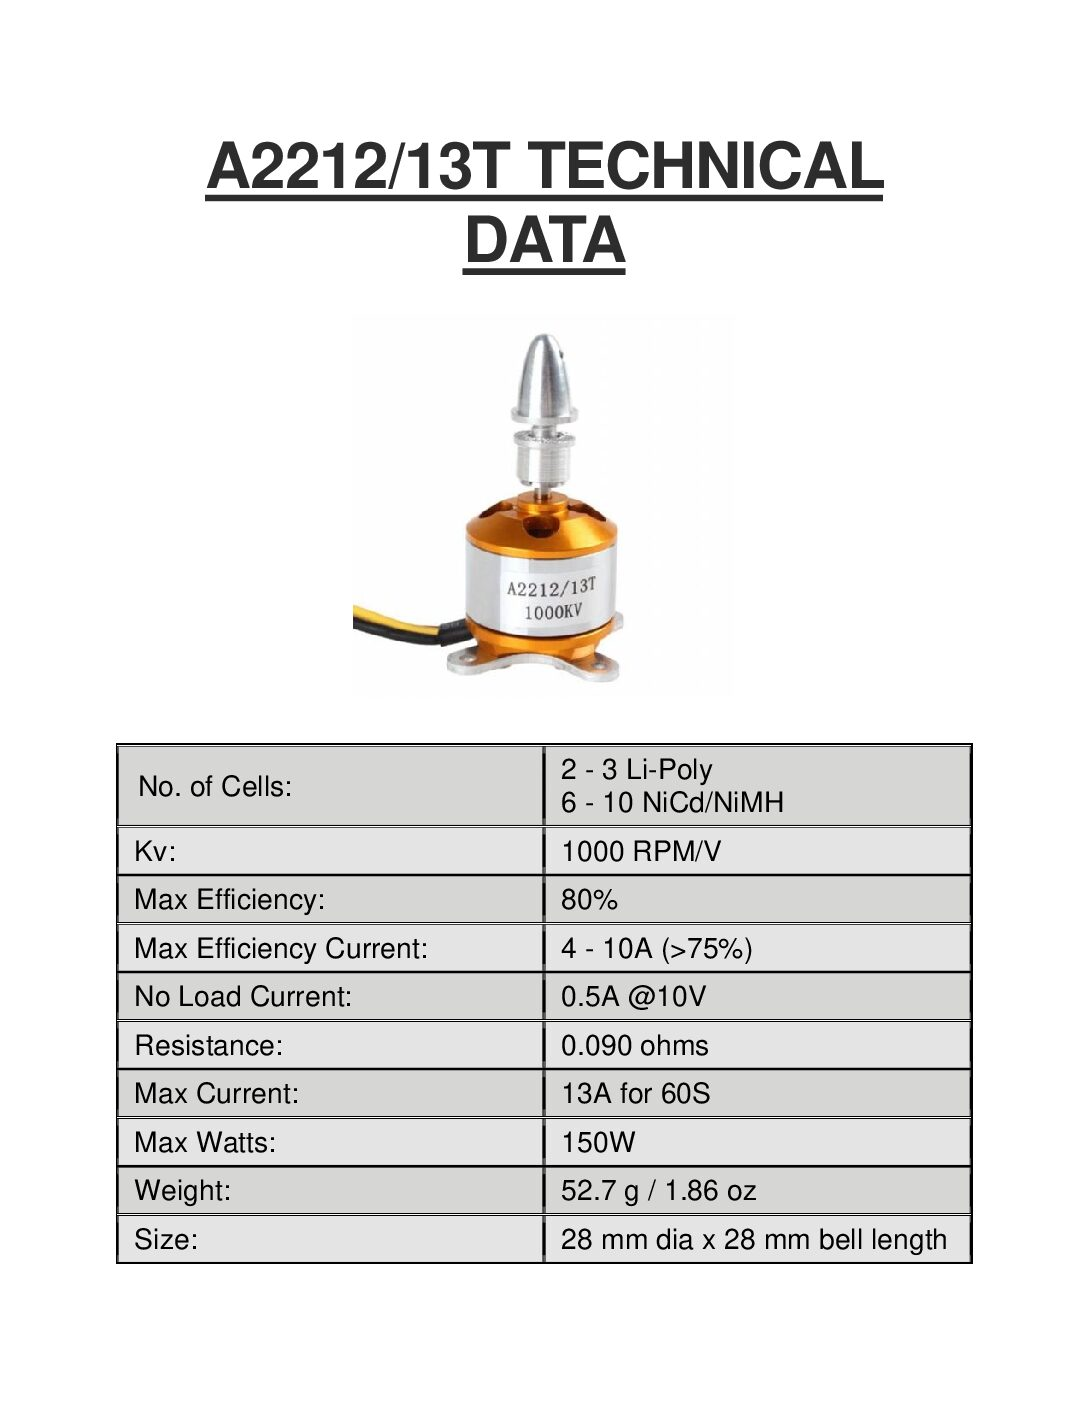
\includegraphics[width=\linewidth]{Figures/motor.jpg}
	\caption[Moteur A2212/13T]{Moteur A2212/13T.}
\end{figure}

\newpage

\subsection{Contrôle PID}

\paragraph{Le contrôle PID (Proportionnel, Intégral, Dérivé) est une méthode courante pour contrôler les systèmes dynamiques en utilisant un retour d'information. Le contrôle PID utilise trois termes pour ajuster la commande du système en fonction de l'erreur, de l'intégrale de l'erreur et de la dérivée de l'erreur.}

\paragraph{Le terme proportionnel ajuste la commande en fonction de l'erreur actuelle, le terme intégral ajuste la commande en fonction de l'accumulation de l'erreur passée et le terme dérivé ajuste la commande en fonction de la variation de l'erreur. Le contrôle PID est largement utilisé dans les applications de contrôle de mouvement, de robotique et de systèmes de contrôle automatique.}

\begin{equation}
	u(t) = K_p e(t) + K_i \int_{0}^{t} e(\tau) \,d\tau + K_d \frac{de(t)}{dt}
\end{equation}

\begin{itemize}
	\item $u(t)$ est la commande du système.
	\item $e(t)$ est l'erreur du système.
	\item $K_p, K_i, K_d$ sont les coefficients du contrôleur PID.
	\item $t$ est le temps.
	\item $\tau$ est le temps de l'intégrale.
	\item $de(t)/dt$ est la dérivée de l'erreur.
	\item $\int_{0}^{t} e(\tau) \,d\tau$ est l'intégrale de l'erreur.
\end{itemize}

\begin{figure}[!htpb]
	\centering
	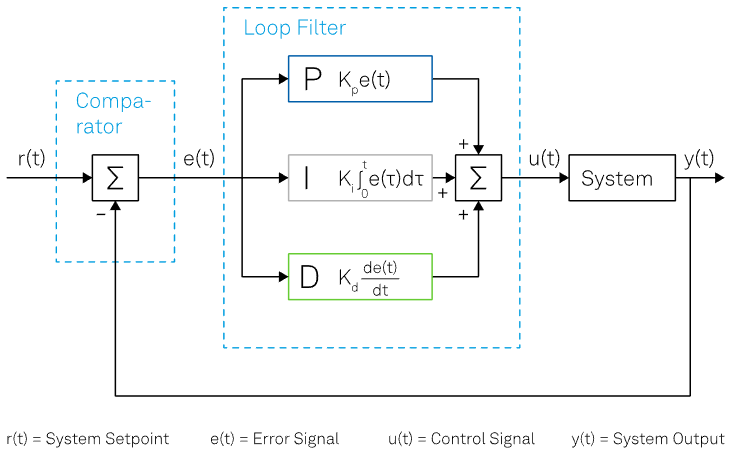
\includegraphics[width=\linewidth]{Figures/pid.png}
	\caption[Contrôle PID]{Contrôle PID.}	
\end{figure}
